\documentclass[12pt,Letter]{article}
%\usepackage[margin=3cm]{geometry}
\usepackage{listings}
\usepackage{graphicx}
\usepackage{float}
\usepackage{color}
\usepackage{tabularx}
\usepackage{adjustbox}
%\usepackage{tikz}
\usepackage[justification=centering]{caption}
%\usetikzlibrary{shapes.geometric,arrows}
%\renewcommand{\lstlistingname}{\textbf{Program}}
\newcommand{\sanper}{\textsc{sanper-1 elu}}
%setting up flowcharts
%\tikzstyle{startstop} = [rectangle, rounded corners, minimum width=3cm, minimum height = 1cm, text centered, draw=black, fill=red!30]

%\tikzstyle{process} = [rectangle, minimum width=3cm, minimum height = 1cm, text centered, text width = 3cm, draw=black, fill=orange!30]

%\tikzstyle{decision} = [diamond,  minimum width=1cm, minimum height = .5cm, text centered, text width = 2cm, draw=black, fill=green!30]

%\tikzstyle{arrow} = [thick, ->,>=stealth]

\definecolor{mygreen}{rgb}{0,0.6,0}
\definecolor{mygray}{rgb}{0.5,0.5,0.5}
\definecolor{mymauve}{rgb}{0.58,0,0.82}

\lstset{ %
	backgroundcolor=\color{white},   % choose the background color; you must add \usepackage{color} or \usepackage{xcolor}
	basicstyle=\footnotesize,        % the size of the fonts that are used for the code
	breakatwhitespace=false,         % sets if automatic breaks should only happen at whitespace
	breaklines=true,                 % sets automatic line breaking
	captionpos=b,                    % sets the caption-position to bottom
	commentstyle=\color{mygreen},    % comment style
	deletekeywords={...},            % if you want to delete keywords from the given language
	escapeinside={\%*}{*)},          % if you want to add LaTeX within your code
	extendedchars=true,              % lets you use non-ASCII characters; for 8-bits encodings only, does not work with UTF-8
%	frame=single,                    % adds a frame around the code
	keepspaces=true,                 % keeps spaces in text, useful for keeping indentation of code (possibly needs columns=flexible)
	keywordstyle=\color{blue},       % keyword style
	language=[Motorola68k]Assembler, % the language of the code
	morekeywords={*,...},            % if you want to add more keywords to the set
	numbers=left,                    % where to put the line-numbers; possible values are (none, left, right)
	numbersep=5pt,                   % how far the line-numbers are from the code
	numberstyle=\small\color{mygray}, % the style that is used for the line-numbers
	rulecolor=\color{black},         % if not set, the frame-color may be changed on line-breaks within not-black text (e.g. comments (green here))
	showspaces=false,                % show spaces everywhere adding particular underscores; it overrides 'showstringspaces'
	showstringspaces=false,          % underline spaces within strings only
	showtabs=false,                  % show tabs within strings adding particular underscores
	stepnumber=1,                    % step between two line-numbers. If it's 1, each line will be numbered
	stringstyle=\color{mymauve},     % string literal style
	tabsize=2                  % sets default tabsize to 2 spac                  % show the filename of files included with \lstinputlisting; also try caption instead of title
}

\begin{document}

\begin{titlepage}
	\begin{center}
		
		
		% Upper part of the page. The '~' is needed because \\
		% only works if a paragraph has started.
		\vfill
		
		\textsc{\LARGE Experiment 7: Parallel Interfacing Using the Peripheral Interface Adapter (PIA)}\\[1.5cm]
		
		\Large Adam Sumner\\[0.5cm]
		
		\Large Illinois Institute of Technology\\[0.5cm]
		
		\Large ECE 441-01\\[0.5cm]	
		% Author and supervisor
		\noindent
		\vfill
		\large \textbf{Lab Date:} April 14th, 2015\hfill
		\large \textbf{Due Date:} April 28th, 2015
		% Bottom of the page
		
		
	\end{center}
\end{titlepage}

\section{Introduction}
The purpose of this experiment is to introduce the student to the peripheral interface adapter IC (PIA, MC6821), the MC68K's Synchronous Cycle, and the MC68K's Interrupt Generation Mechanism. A circuit will be designed and constructed to allow the user to input a character into the PIA so that the PIA will output the received input back to the user.
\section{Background}
\subsection{The Peripheral Interface Adapter (PIA)}
The Peripheral Interface Adapter or PIA, provides a general purpose means of interfacing
peripheral equipment to the MC68000. This integrated circuit is capable of interfacing a microprocessor to peripheral devices through two 8-bit bi-directional peripheral data buses (PA0 to PA7, and PB0 to PB7) and four control lines (CA1, CA2, CB1, and CB2)\cite{expman}.

The functionality of the PIA is programmable by the CPU during initialization of the system. Each of the data lines can be programmed to perform either as an input or output line, and each of the control lines can programmed to operate in one of several modes\cite{expman}.

\subsection{Internal Architecture}
The PIA occupies four consecutive locations in the CPU's memory map. The PIA contains six internal registers, three for Port A, and three for Port B. The Register Select Lines(RS1,RS0) are used to select one of the four registers inside the PIA. Table \ref{tab:regselect} shows this relationship.
\begin{table}[H]
	\centering
	\begin{tabular}{c c c c|c}
		CR2	&	CRB2	&	RS1	&	RS0	&	PIA Register Selected \\
		\hline  \hline
		0 	&	X	&	0	&	0	&	Data Direction Register, Port A \\
		1	&	X	&	0	&	0	&	Peripheral Data Register, Port A \\
		X	&	X	&	0	&	1	&	Control Register, Port A \\
		X	&	0	&	1	&	0	&	Data Direction Register, Port B \\
		X	&	1	&	1	&	0	&	Peripheral Data Register, Port B \\
		X	&	X	&	1	&	1	&	Control Register, Port B
		
	\end{tabular}
	\caption{Register Selection}
	\label{tab:regselect}
\end{table}
\subsubsection{Registers}
\begin{enumerate}
	\item \textit{Data Direction Register (DDRA or DDRB)}: 
	
	\vspace{.2cm}
	This register programs each of the eight peripheral data lines (PA0 $\to$ PA7 or PB0 $\to$ PB7) to act as either an input or an output. Setting a bit equal to “1” defines its corresponding peripheral data line to be an output, while setting a bit equal to “0” defines its corresponding peripheral data line to be an input\cite{expman}.
	
	\item \textit{Peripheral Data Register (PDRA or PDRB)}:
	
	\vspace{.2cm}
	\underline{Inputs}
	
	\vspace{.2cm}
	The signals from the peripheral data lines are input into this register. The CPU may then read this register to determine the status of the peripheral data lines\cite{expman}.
	
	\vspace{.2cm}
	\underline{Outputs}
	
	\vspace{.2cm}
	The data written to this register by the CPU will appear on the peripheral data lines that are programmed as outputs. A ``1" written into this register by the CPU causes a ``high" level signal to appear on the corresponding peripheral data line. Similarly, a ``0" written into this register by the CPU causes a ``low" level signal to appear on the corresponding peripheral data line\cite{expman}.
	
	\item \textit{Control Register (CRA or CRB)}:
	
	\vspace{.2cm}
	This register allows the CPU to configure the operation of the two peripheral control lines, CA1 and CA2 or CB1 and CB2. This register also allows the CPU to enable interrupt lines and monitor the status of the interrupt flags. Bit 2 of this register is used along with select lines (RS1, RS0) to determine whether the Data Direction Register or the Peripheral Data Register is to be accessed\cite{expman}.
\end{enumerate}

\subsection{MC68000 Synchronous Bus Cycle}
In order for the 68000 to interface to 6800 type peripherals, the 68000 modifies its bus cycle to meet the 6800 bus cycle timing requirements whenever a 6800 type device is selected. This feature is possible because both types of processors use memory-mapped I/O. Three signals are used to achieve compatibility. They are:
\begin{enumerate}
	\item \textit{Enable} (E)
	
	\vspace{.2cm}
	This corresponds to the E signal that exists in 6800 systems. It's the bus clock used by 6800 peripherals to synchronize data transfers. It is a free-running clock that is one tenth the frequency of the 68000's clock signal. It has a 60/40 duty cycle.
	
	\item \textit{Valid Peripheral Address} ($\overline{VPA}$)
	
	\vspace{.2cm}
	This input signal informs the 68000 that the address on the bus is the address on the 6800 device and that the bus should conform to the E clock transfer characteristics of the 6800 bus. $\overline{VPA}$ is derived by decoding the address bus, and qualifying it with \textit{Address Strobe} ($\overline{AS}$)
	
	\item \textit{Valid Memory Address} ($\overline{VMA}$)
	
	\vspace{.2cm}
	This output signal notifies any 6800 peripherals that the address on the address bus is valid, and that the 68000 is synchronized to the Enable (E) signal. The $\overline{VMA}$ signal is used as part of the chip select circuitry for the peripheral. This ensures that 6800 type peripherals are selected and unselected at the proper time.
\end{enumerate}
\section{Equipment/Procedure}
\subsection{Equipment}
\begin{itemize}
	\item \textsc{SANPER-1 Educational Lab Unit}
	\item Computer with TUTOR software
	\item Open Collector Inverter Gate Chip
	\item NOR Gate Chip
	\item Decoder Chip
	\item PIA Chip
\end{itemize}
\subsection{Procedure}
The first step is to draw a detailed schematic diagram of the hardware to be implemented. Once this is done, the designed hardware is to be built on breadboard strips. After this, the software must be designed. An initialization routine to configure the PIA for:
	\begin{itemize}
		\item Port A lines to be inputs
		\item Port B lines to be outputs
		\item IRQA interrupt to be enabled and asserted by a high to low transition on CA1
		\item Port B to use pulse-mode handshaking
	\end{itemize}
must be written, along with an interrupt service routine that reads the peripheral data on PA0 $\to$ PA7 of Port A and displays the received character on the terminal. Once this is done, a program should be written to continuously read a character from the keyboard and output it to the peripheral data side of Port B of the PIA.
\section{Results}
Below are the results from the experiment. Figure \ref{fig:hardwareimp} shows the physical implementation of the designed hardware, while Figure \ref{fig:output} shows the I/O in action.
\begin{figure}[H]
\centering
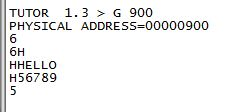
\includegraphics[width=.5\linewidth]{output}
\caption{I/O Demonstration}
\label{fig:output}
\end{figure}

\begin{figure}[H]
\centering
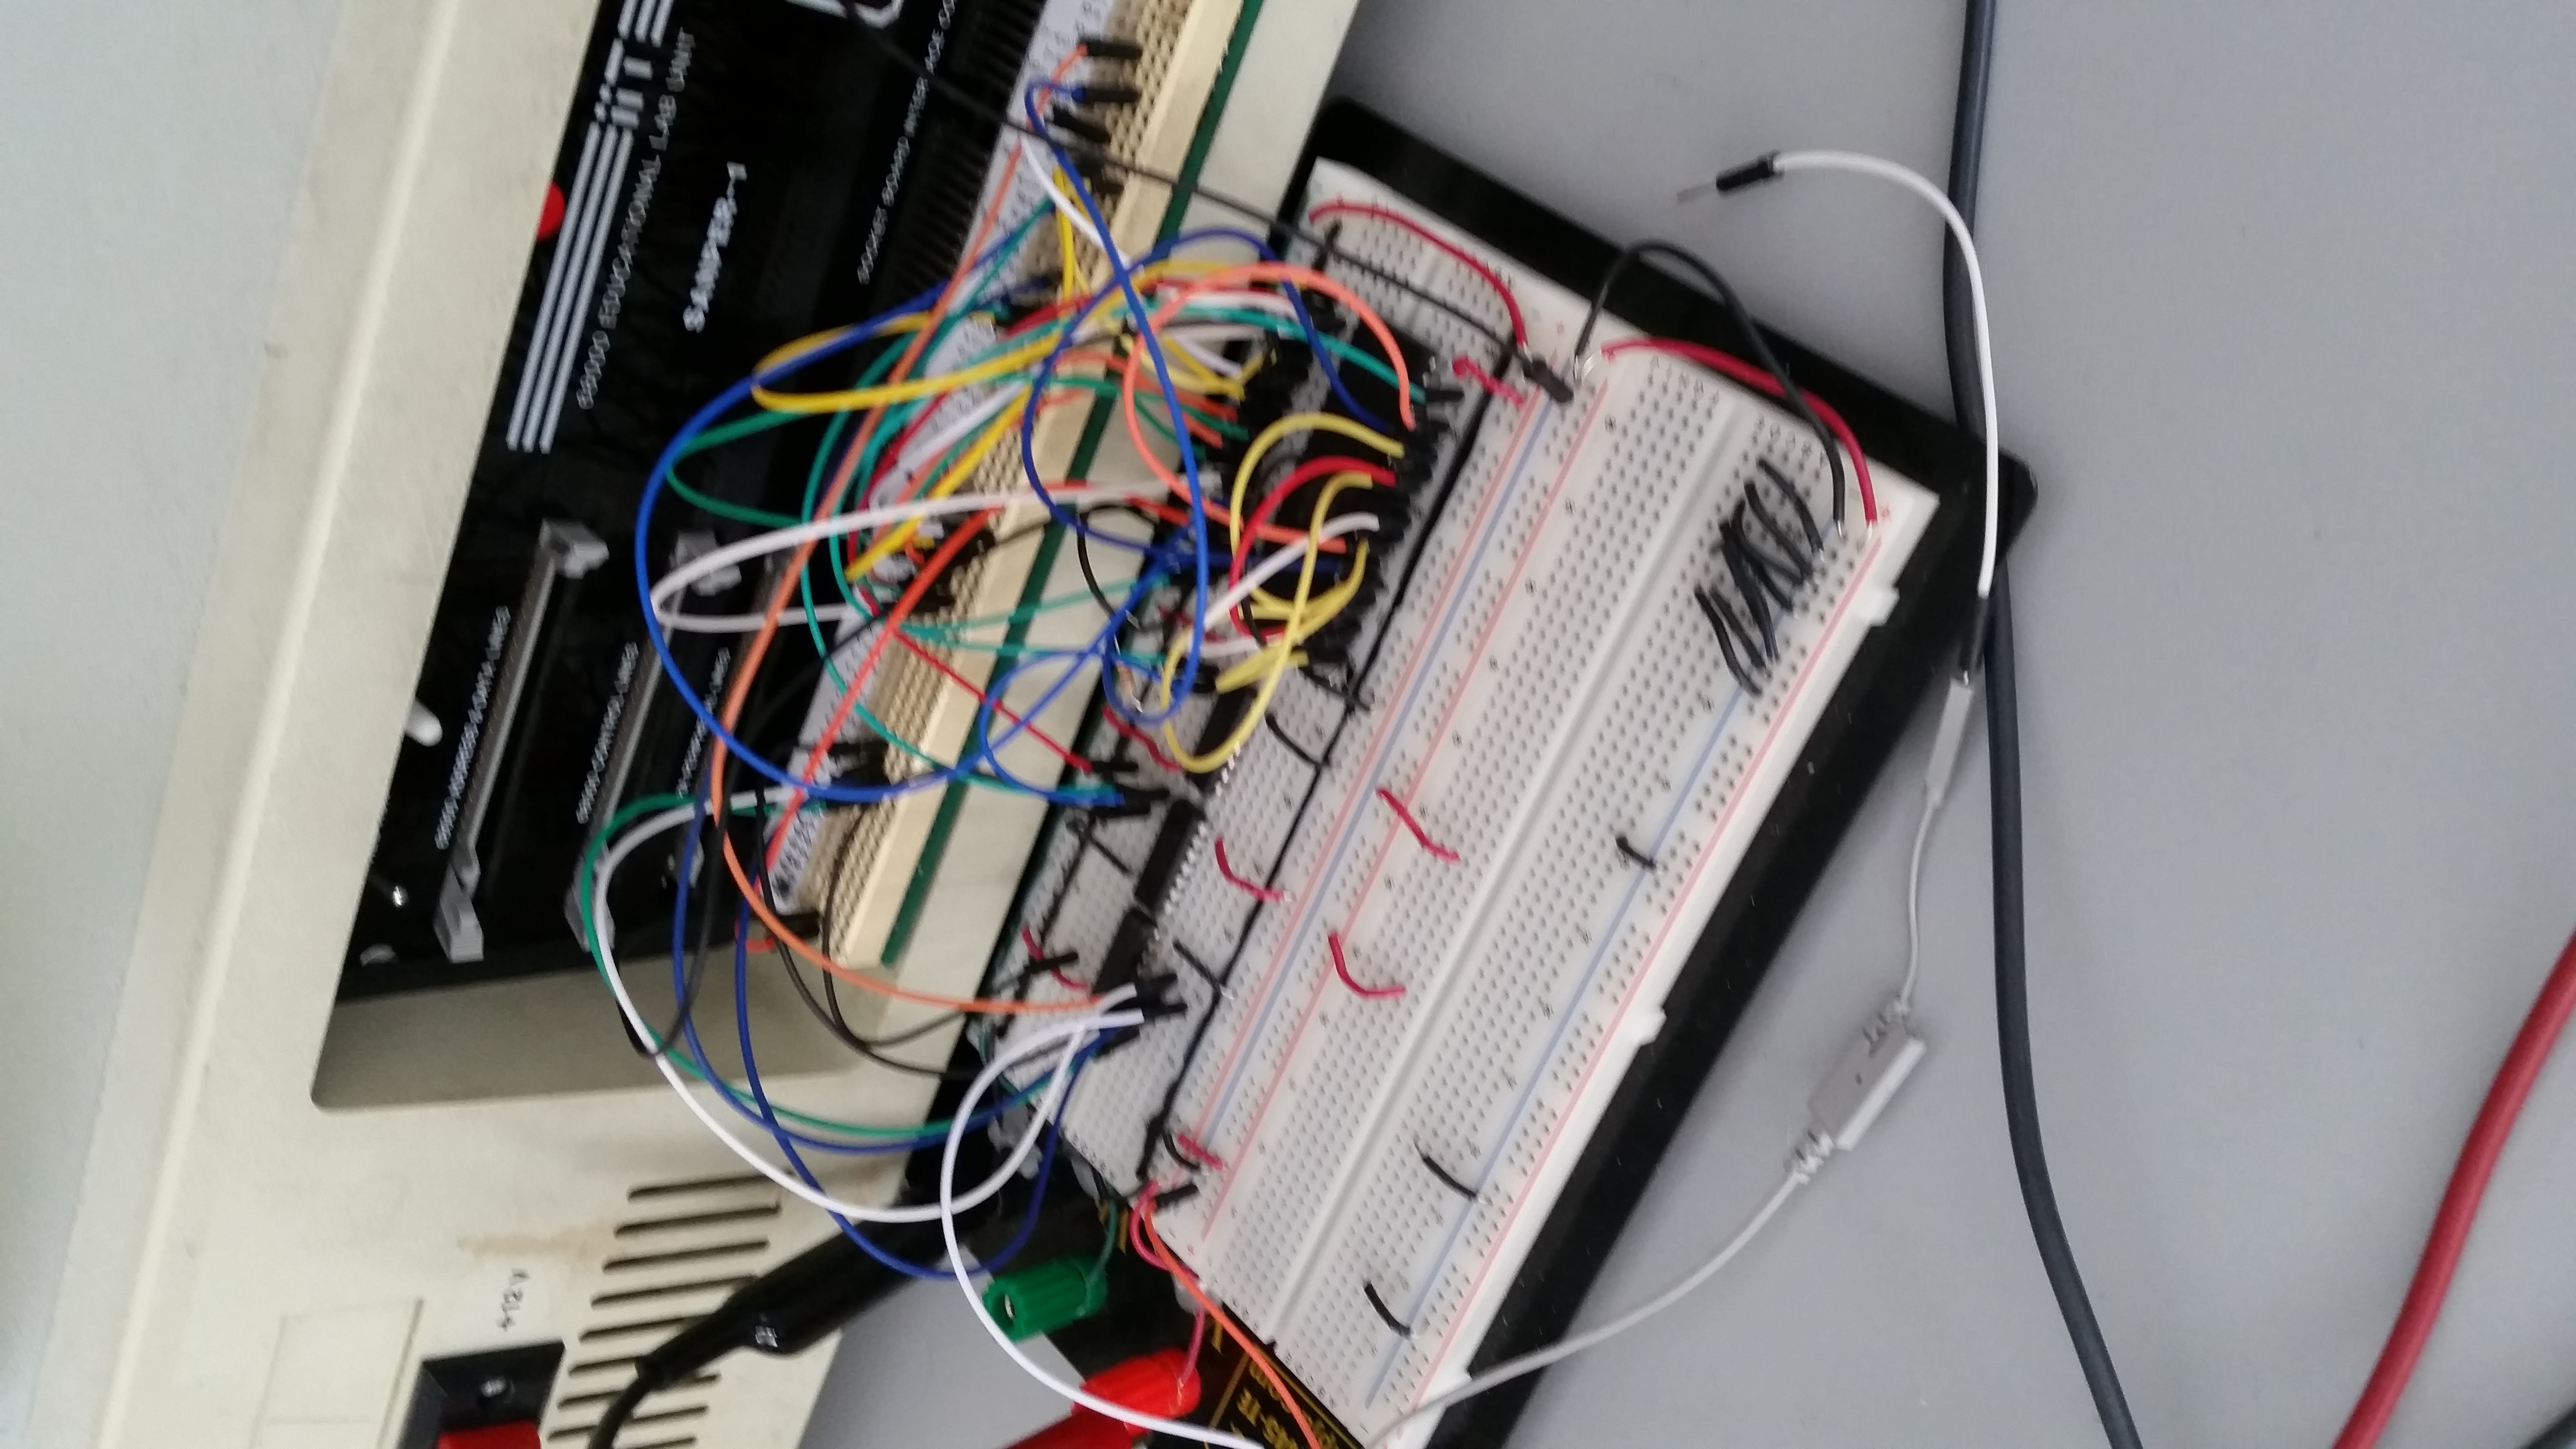
\includegraphics[width=1\linewidth]{20150414_102437}
\caption{Physical Implementation of Circuit}
\label{fig:hardwareimp}
\end{figure}

\section{Discussion}
\subsection{Answers to Discussion Problems}
\begin{enumerate}
	\item Program is located in Section \ref{code}
	\item The hardware schematic is located in Section \ref{sec:hardware}
	\item The PIA used an auto vector interrupt because it cannot generate its own.
	\item The microprocessor has to poll both sides of the status register to determine which side generated the interrupt request
	\item \begin{tabular}{|c|c|c|c|c|}
		\hline 
			IRQA1 & IRQA2 & CA2 Control & DDRA & CA1 Control \\ \hline
			0 & 0 & 1 1 1 & 1 & 11 \\ \hline
	\end{tabular}
	
	~\\
	There are no pending interrupts, CA2 output is always high, PDRA is selected, and rising1 transitions create an unmasked IRQA1 interrupt.
	\item The PIA could be used in an old ATARI 800 computer to provide four joystick ports to the machine, it can be used in an old computer to interface the ASCII keyboard and the display, and it could be of use in machines such as an electric pinball machine.  
	\item ~\\
	
\begin{figure}[H]
\centering
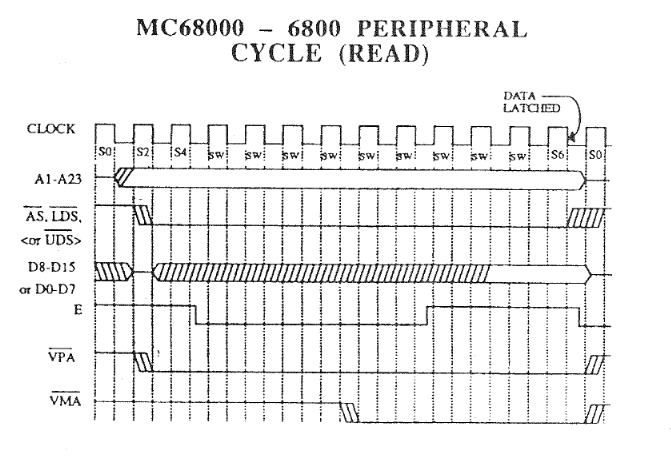
\includegraphics[width=1\linewidth]{bus}
\caption{MC68000 Bus Cycle}
\label{fig:bus}
\end{figure}
\end{enumerate}

\begin{enumerate}
	 \item Address lines stabilize
	 \item $\overline{VPA}, \overline{AS}, \overline{LDS}$, or $\overline{UDS}$ stabilize
	 \item $\overline{VMA}$ stabilizes
	 \item Data lines stabilize
	 \item Data latches
	 \item All lines reset
\end{enumerate}
\section{Conclusion} 
Overall the experiment was a success. The student was successfully introduced to the peripheral interface adapter IC (PIA, MC6821), the MC68K's Synchronous Cycle, and the MC68K's Interrupt Generation Mechanism. Through the design work done in this experiment, these concepts were solidified.
\begin{thebibliography}{1}
	\bibitem{expman} Experiment 7 Lab Manual
	\bibitem{ecbm} Educational Computer Board Manual
	\bibitem{m68k}MC68K User Manual
	\bibitem{sanper}SANPER-1 ELU User Manual
\end{thebibliography}
  

\section{Appendix}
\label{appendix}
\subsection{Code}\label{code}
\lstinputlisting{lab7.X68}
\subsection{Hardware}\label{sec:hardware}
\begin{figure}
\centering
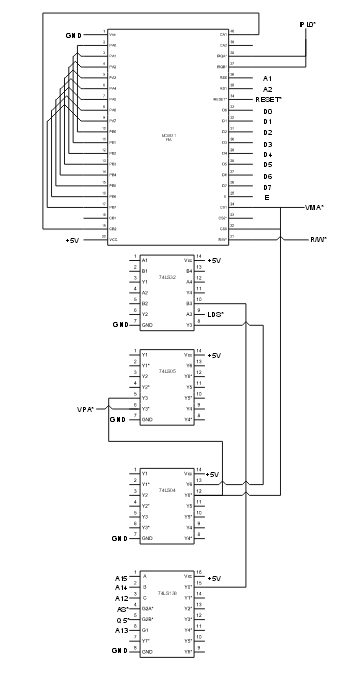
\includegraphics[width=.8\linewidth]{schematic}
\caption{Hardware Schematic for PIA}
\label{fig:schematic}
\end{figure}

\end{document}
